\subsubsection{Análisis de Resultados}
En esta sección presentamos y analizamos los resultados obtenidos en los experimentos de clasificación automática de textos según los niveles del CEFR. El objetivo es comparar el rendimiento de los distintos enfoques evaluados, prompting, prompting con conocimiento lingüístico, modelos libres, privativos y fine-tuning, así como entender en qué condiciones cada estrategia resulta más eficaz. A lo largo del análisis mostramos cómo las aproximaciones basadas en fine-tuning superan sistemáticamente al resto de alternativas, y discutimos los factores que explican estas diferencias.\\

\noindent\textbf{Comparación general entre modelos con y sin fine-tuning}\\
En la Figura \ref{fig:finetuning} se observa una diferencia clara y consistente entre el modelo ajustado mediante fine-tuning y aquellos evaluados únicamente con estrategias de prompting (incluyendo prompting pedagógico, descriptores CEFR y prompting con conocimiento lingüístico).

El modelo con fine-tuning alcanza niveles de precisión considerablemente superior, lo que evidencia la importancia de adaptar los LLMs preentrenados al dominio específico de clasificación CEFR.\\

\begin{figure*}[]
  \centering
  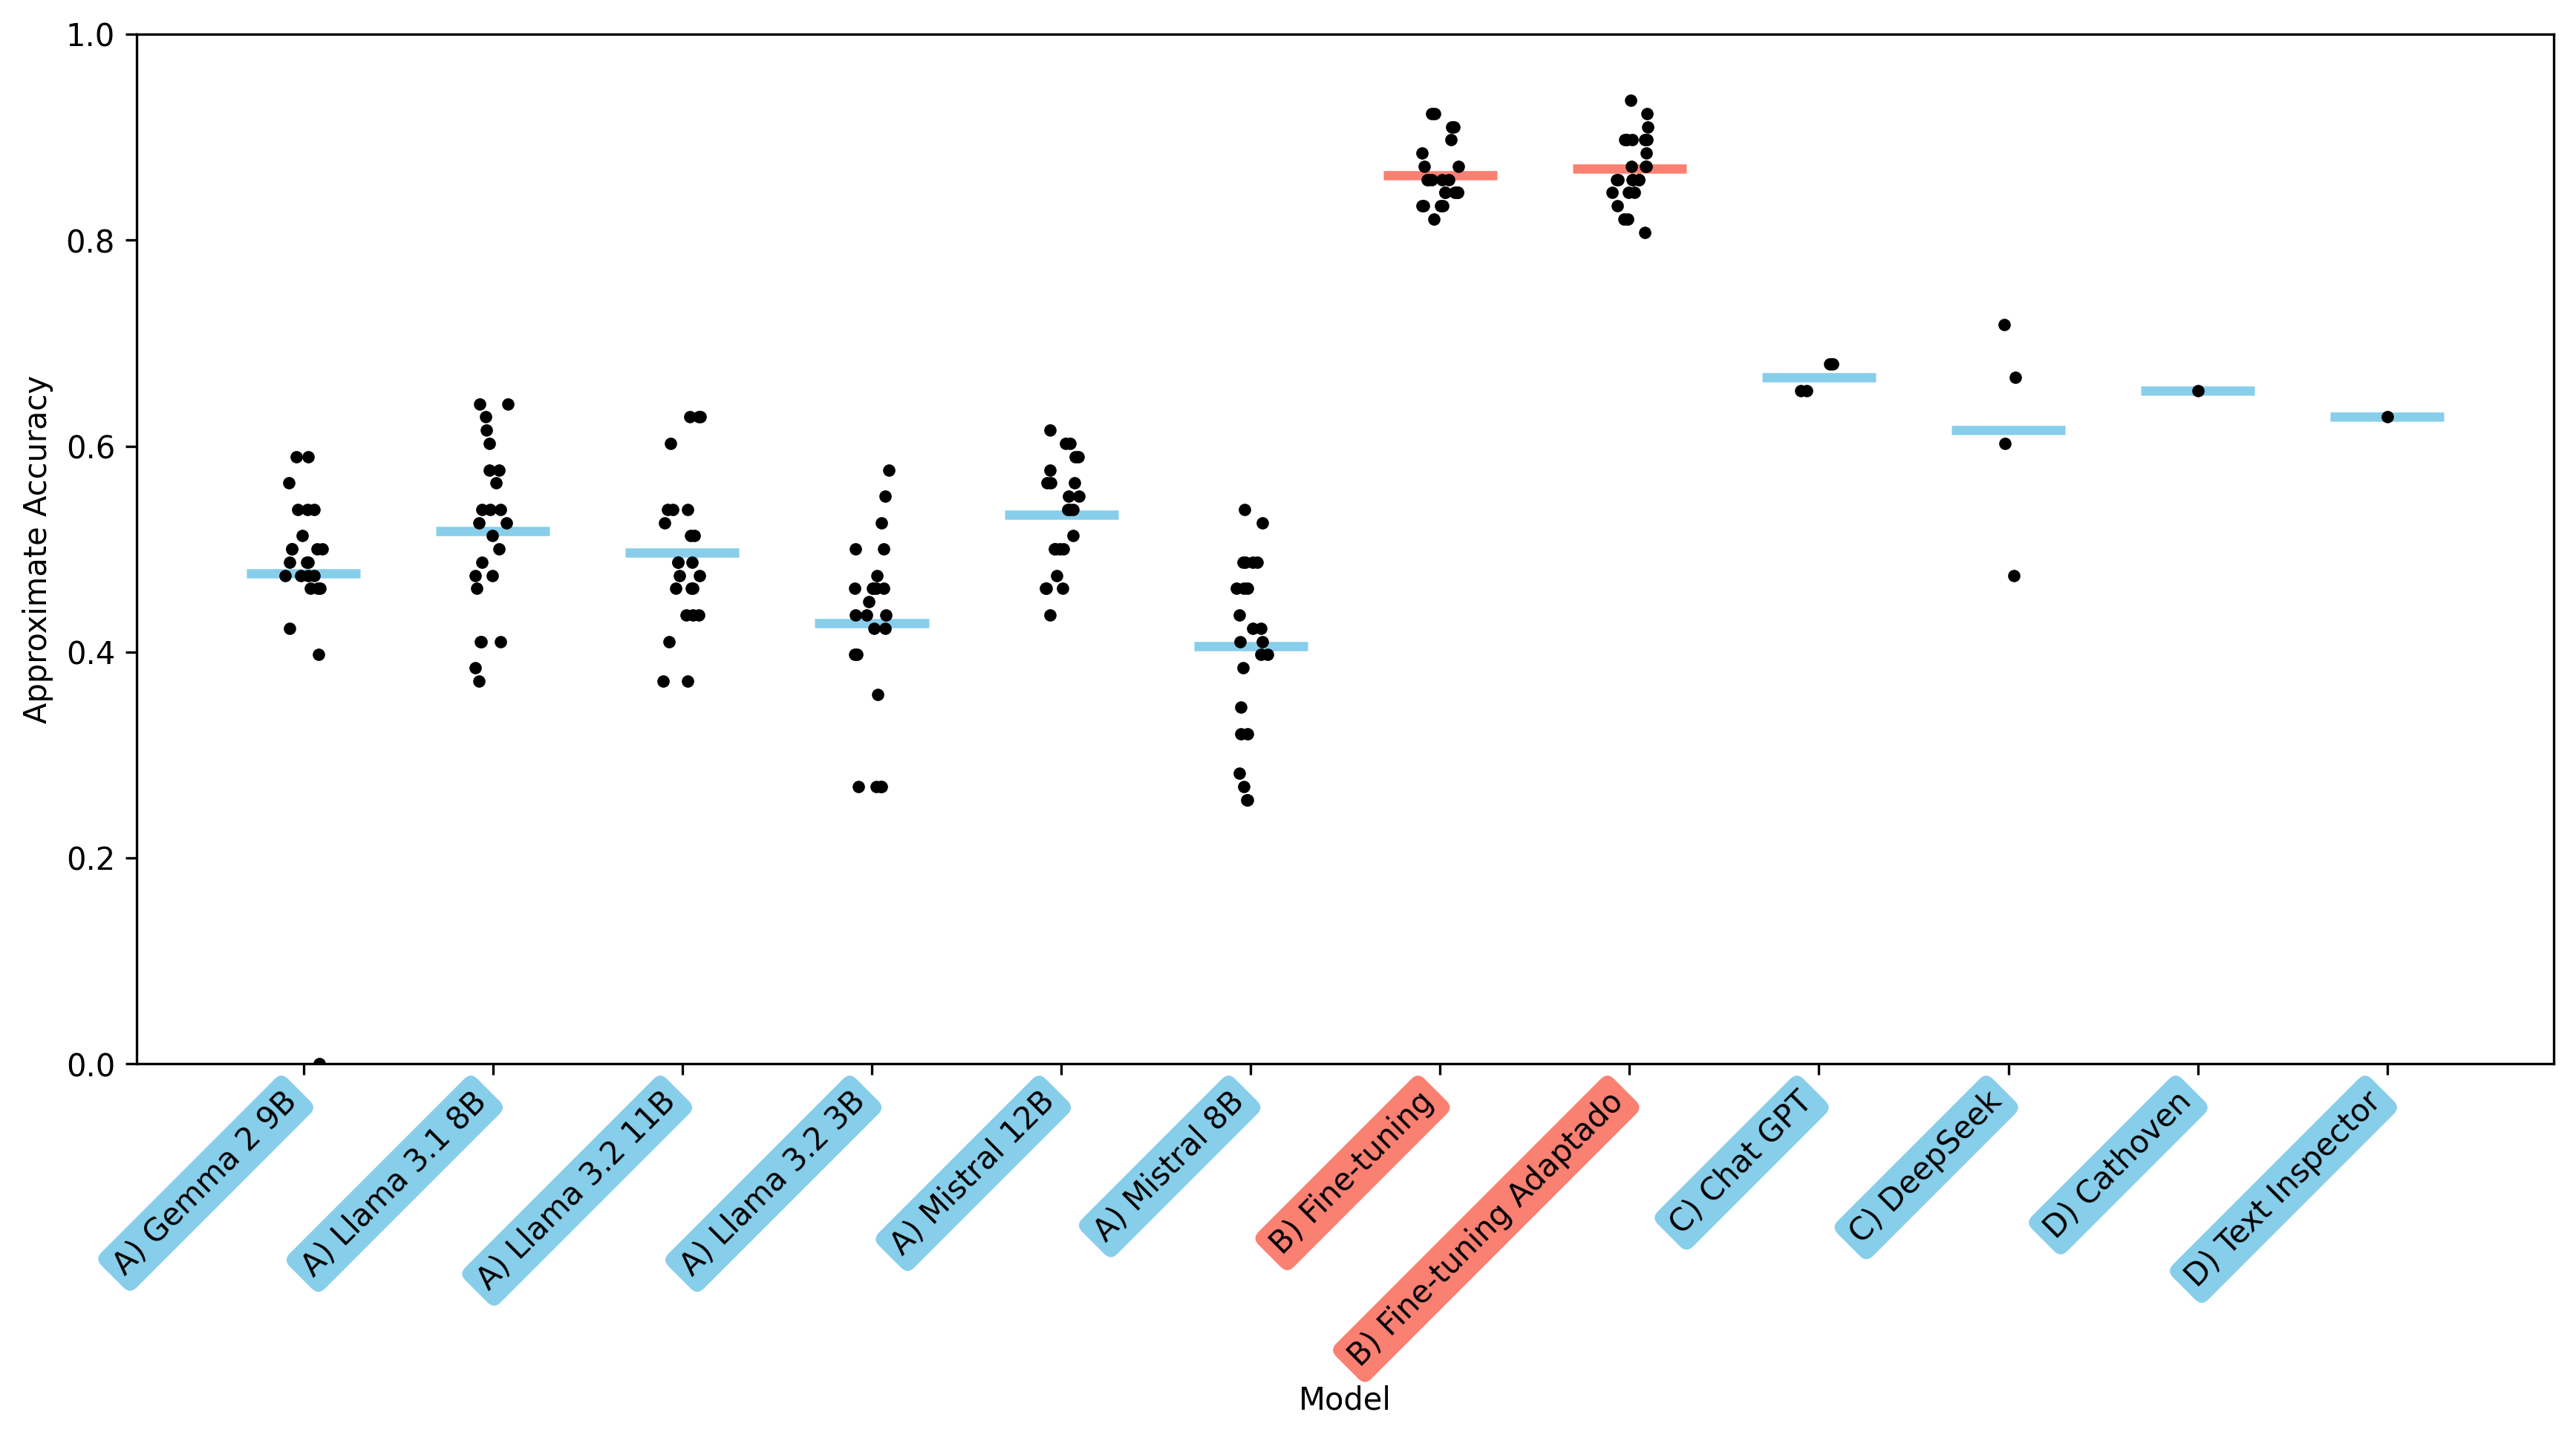
\includegraphics[width=\textwidth]{Graficos Tesis/custom_dataset_evaluacion_con_finetuning_vs_sin_Accuracy_aprox.png}
  \caption{Aproximated Acuraccy de los modelos sin finetuning (celeste) vs modelos con finetuning (rojo), con promedio de todos los prompts usados}
  \label{fig:finetuning}
\end{figure*}

\noindent\textbf{Modelos privativos vs. modelos open-source}\\
La Figura \ref{fig:privativos} presenta una comparación directa entre los modelos libres y los modelos privativos ChatGPT y DeepSeek. Debido a restricciones de uso y costo, estos últimos solo se evaluaron en los prompts 15 a 18, correspondientes a prompting con 2 ejemplos seleccionados por docentes.

Los resultados muestran que los modelos privativos exhiben un rendimiento más estable y ligeramente superior respecto a los modelos open-source sin fine-tuning. Sin embargo, esta ventaja no es marcada: dos de los modelos libres (LLaMA 3.1 8B y LLaMA 3.2 11B) alcanzan precisiones comparables, confirmando que las arquitecturas abiertas pueden resultar competitivas.

El mejor modelo de toda la comparación continúa siendo el modelo con fine-tuning, presentado como línea de referencia en la figura.

Es importante destacar que estos resultados fueron obtenidos exclusivamente sobre la partición eval del Custom dataset, lo que permitió asegurar condiciones comparables entre todos los modelos involucrados.\\

\begin{figure*}[]
  \centering
  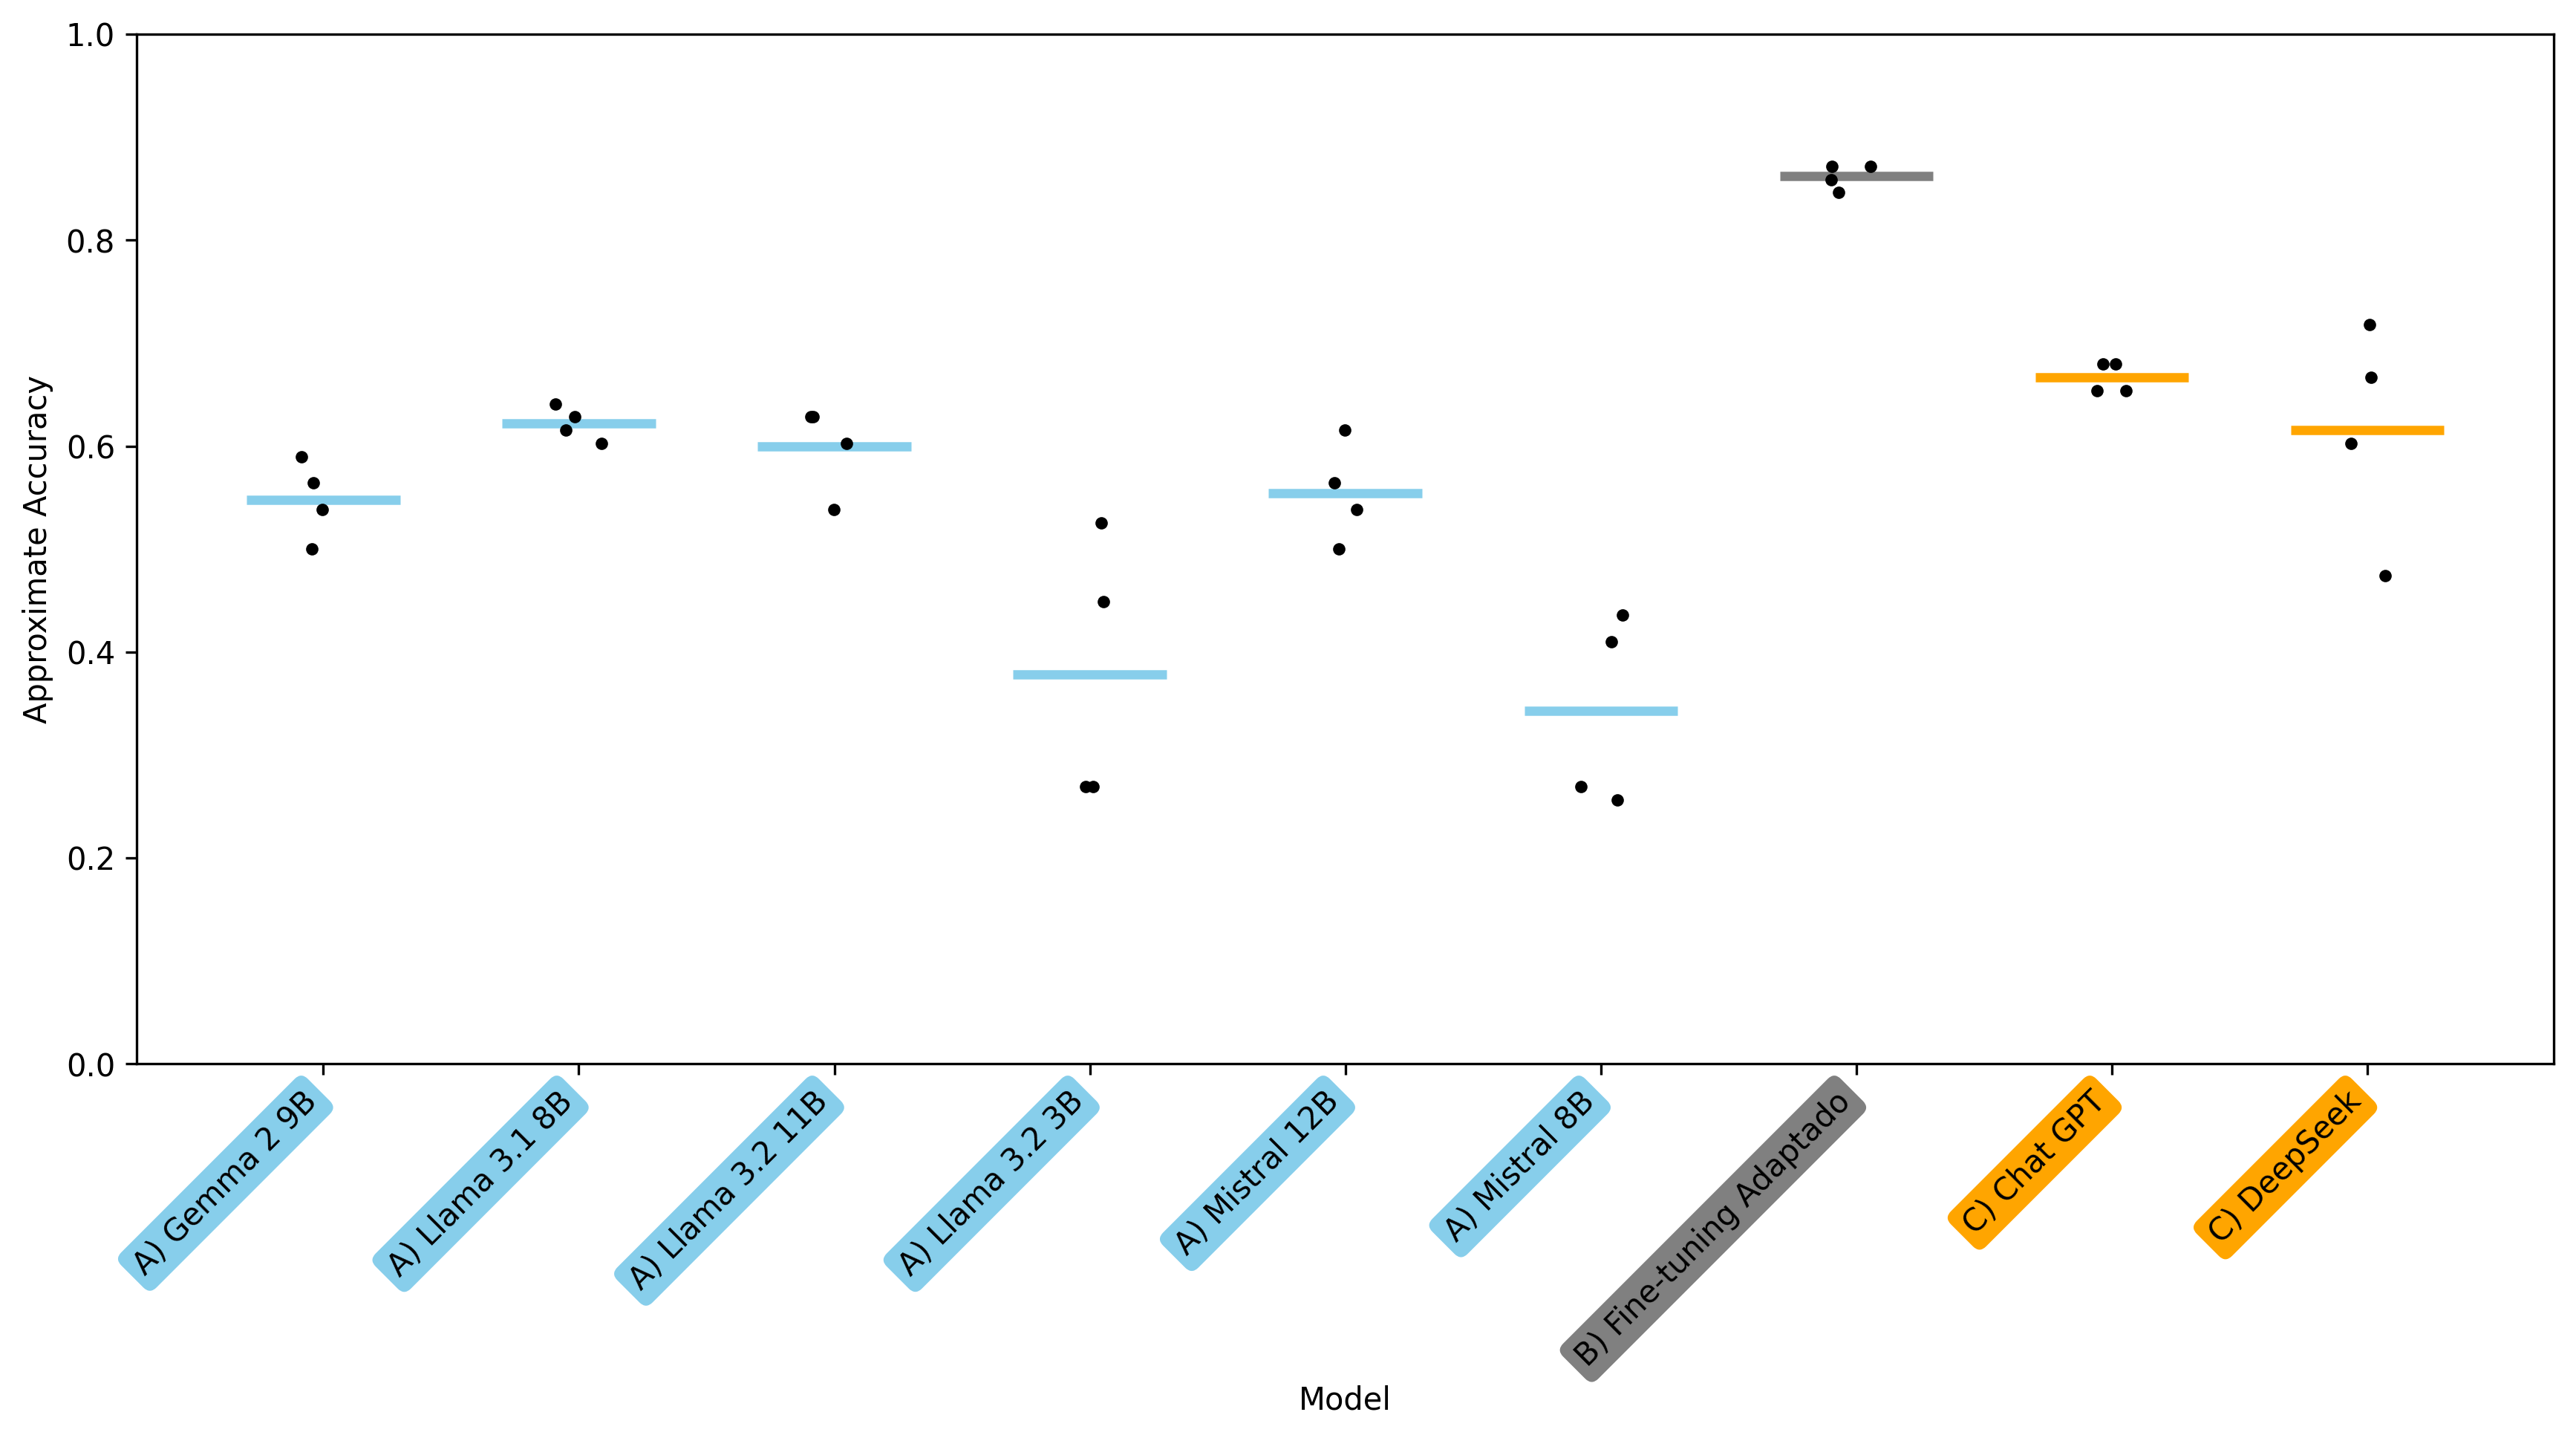
\includegraphics[width=\textwidth]{Graficos Tesis/custom_dataset_evaluacion_privativo_vs_libre_acuraccy_aprox.png}
  \caption{Aproximated Acuraccy de los modelos libres (celeste) vs modelos privativos (naranja), con promedio de los prompts 15 a 18}
  \label{fig:privativos}
\end{figure*}

\noindent\textbf{Comparación entre modelos open-source}\\
En la Figura \ref{fig:libres} se comparan los modelos libres utilizando la partición combinada train + eval. Esta decisión permitió aumentar la cantidad de textos en la evaluación, reduciendo la varianza en los indicadores de desempeño.

Una de las principales observaciones es que los valores promedio de accuracy se ubican dentro del rango 0.45–0.55. Luego LLaMA 3.1 8B y Mistral 12B obtienen las mejores medias de precisión. Ademas Mistral 12B presenta menor dispersión en los resultados, reflejando un comportamiento más estable y por ultimo LLaMA 3.1 8B alcanza algunos de los valores máximos más altos de toda la comparación.

En función de estos resultados y considerando además su menor tamaño y requerimientos computacionales, se seleccionó el modelo LLaMA 3.1 8B como candidato principal para aplicar fine-tuning.\\

\begin{figure*}[]
  \centering
  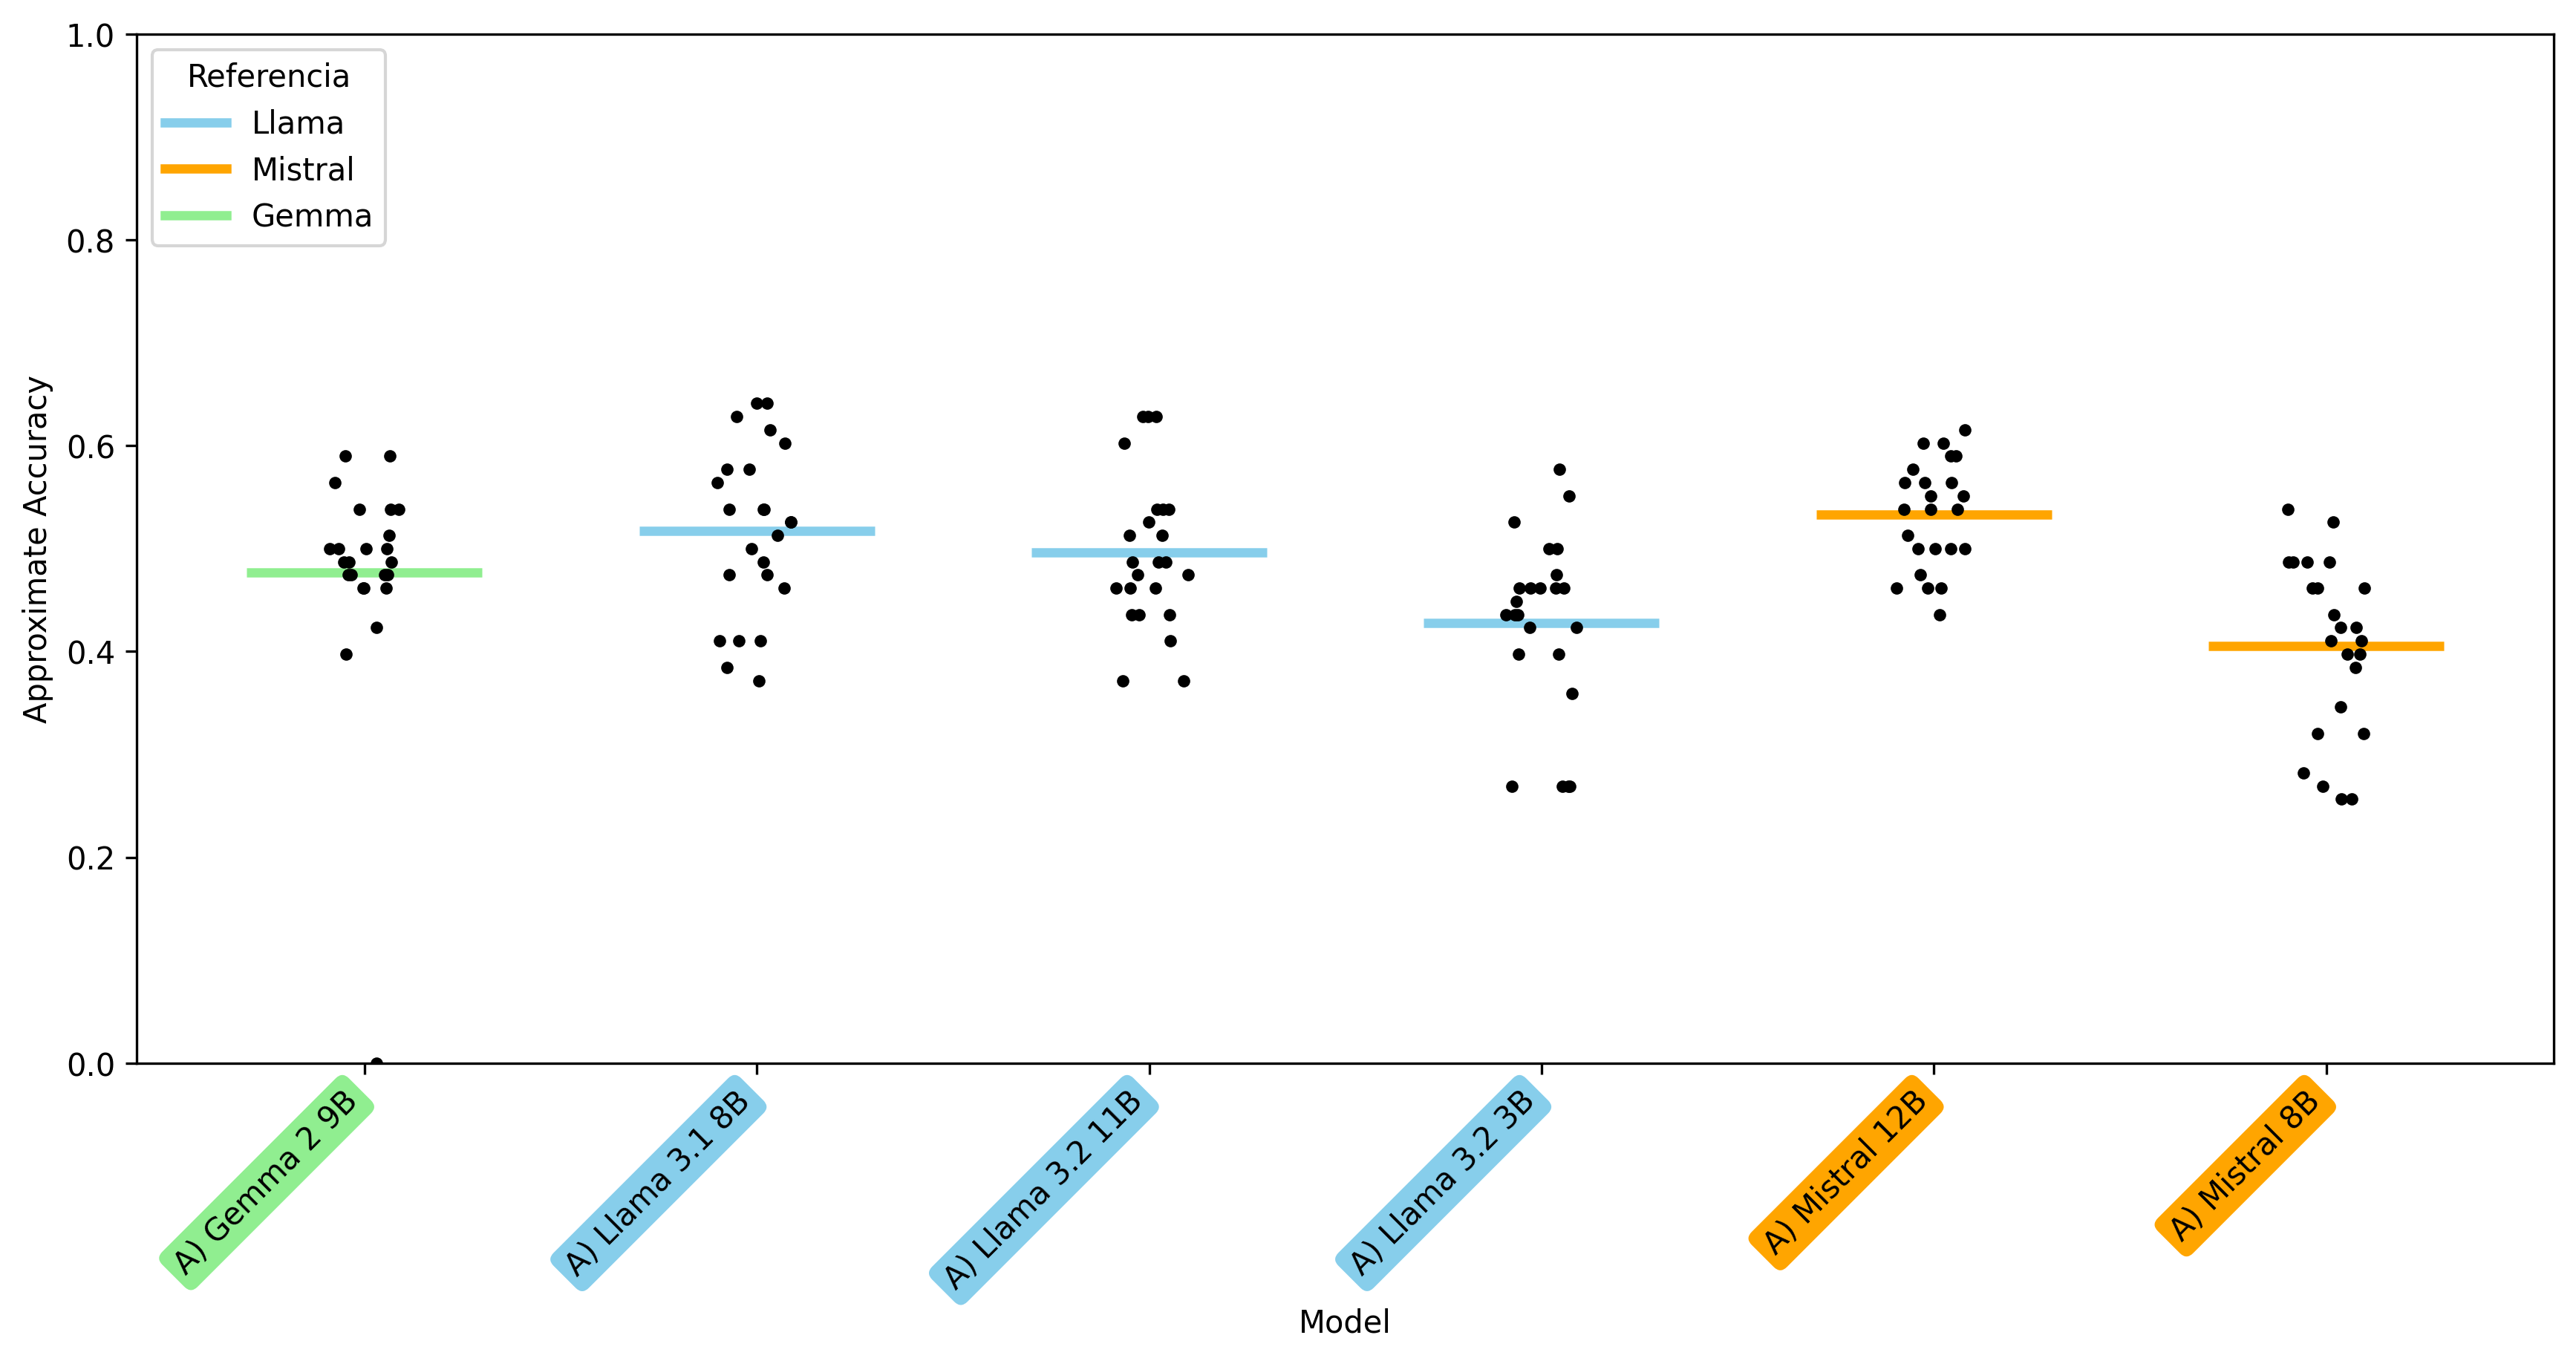
\includegraphics[width=\textwidth]{Graficos Tesis/custom_dataset_evaluacion_differencias_entre_libres_acuracy_aprox.png}
  \caption{Aproximated Acuraccy de los modelos libres, con promedio de todos los prompts}
  \label{fig:libres}
\end{figure*}

\todo{sacar referencia de la imagen}

\noindent\textbf{Influencia del tipo de prompt y longitud del prompt}\\
La Figura \ref{fig:todos_los_modelos} y \ref{fig:modelos_ind} muestra el desempeño de los modelos comparando distintas estrategias experimentales (0-shot, 1-shot, 2-shot, prompting pedagógico, prompting con conocimiento lingüístico y variantes con corrección de sesgo).

Se puede obsevar que los modelos con fine-tuning mantienen ventaja incluso frente a prompts largos. Aunque la longitud del prompt introduce variabilidad, los modelos ajustados continúan obteniendo mejores resultados que cualquier configuración sin entrenamiento adicional.

La longitud excesiva del prompt puede degradar el rendimiento. Especialmente en prompting con conocimiento lingüístico, que requiere instrucciones más extensas y algunos modelos muestran una caída notable, posiblemente originada por efectos adversos en los mecanismos de atención (“olvido” parcial del contenido relevante). Este comportamiento se observa con mayor fuerza en modelos medianos como Mistral 3B o Gemma 2 9B.

Ademas para algunos prompt particulares se puede ver una caida en el rendimiento en comparacion a prompts similares, por ejemplo para el prompt 11 (1-shot con correccion de sesgo) se puede observar que en todos los modelos libres (salvo Gemma 2 9B y Mistral 12B) tienen esta caida.

Las tendencias dependen del modelo.
\begin{itemize}
    \item LLaMA 3.1 8B: leve mejora progresiva de 0-shot → 1-shot → 2-shot.
    \item LLaMA 3.2 11B: comportamiento similar, aunque con menor gradiente de mejora.
    \item Mistral 12B: los prompts pedagógicos no superan al rendimiento 0-shot.
    \item Gemma 2 9B: alta sensibilidad al tamaño del prompt; en el experimento 23 obtiene accuracy 0 debido a una ventana de contexto insuficiente.
    \item Mistral 3B: empeora al incrementar la complejidad del prompt.
\end{itemize}

Estos resultados sugieren que, para algunos modelos, proporcionar más información no necesariamente mejora la predicción; en ciertos casos incluso introduce ruido estructural o saturación de contexto.\\

\begin{figure*}[]
  \centering
  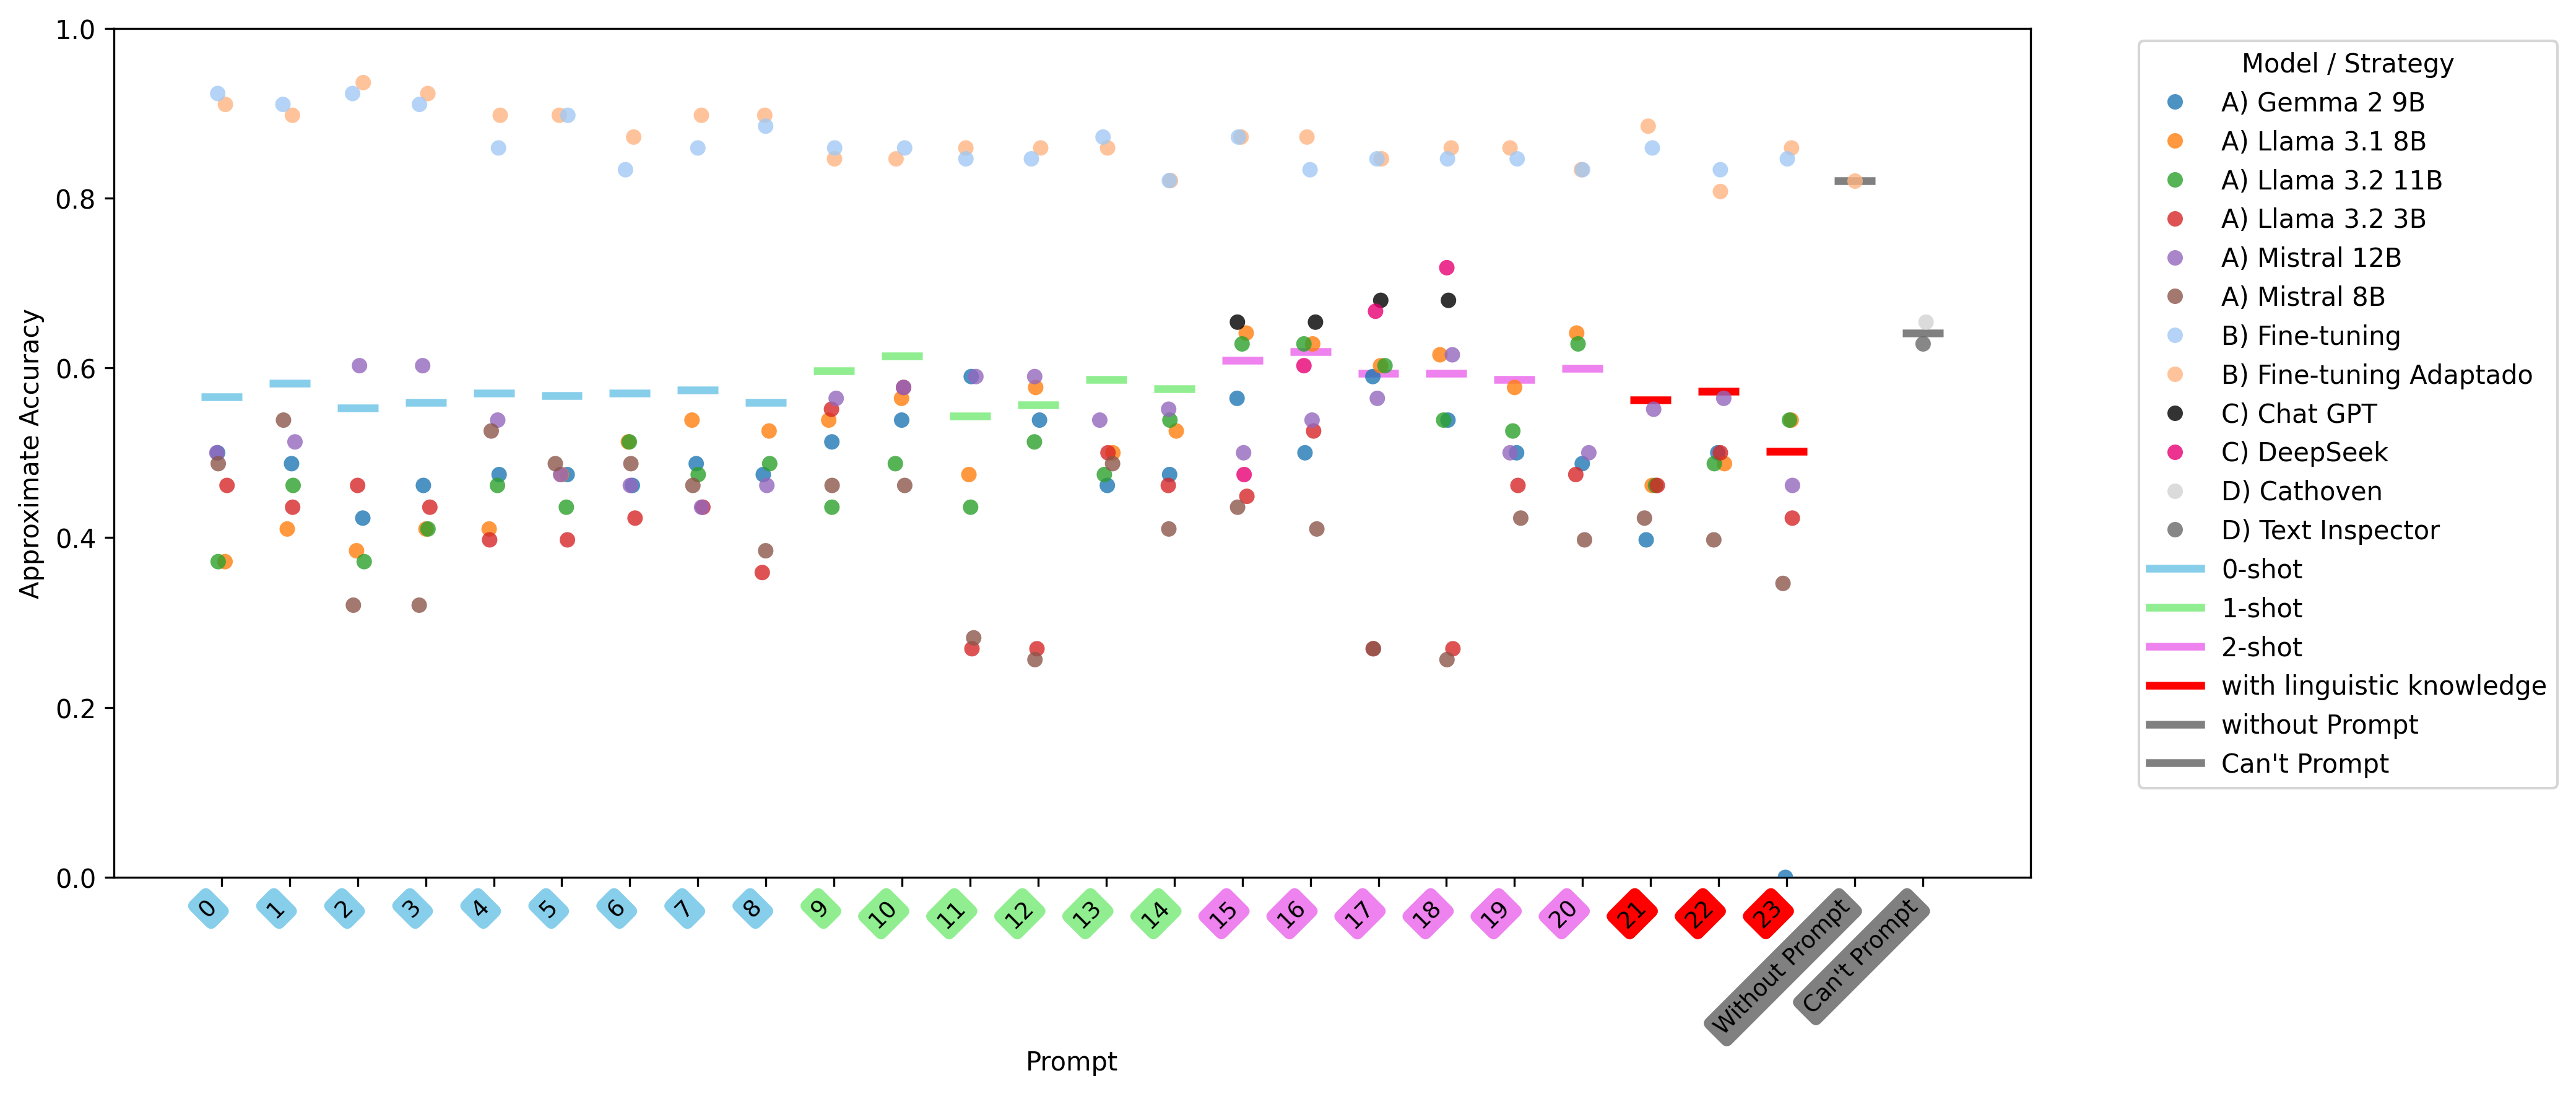
\includegraphics[width=\textwidth]{Graficos Tesis/custom_dataset_evaluacion_experimentos_Accuracy_aprox.png}
  \caption{Aproximated Acuraccy de todos los experimentos realizados, con promedio de todos los modelos segun los prompts. Los resultados fueron coloreados segun el tipo de modelo, colores nitidos modelos libres, colores claros modelos con finetuning, colores oscuros modelos privativos y colores grises herramientas.}
  \label{fig:todos_los_modelos}
\end{figure*}

\begin{figure*}[]
  \centering
  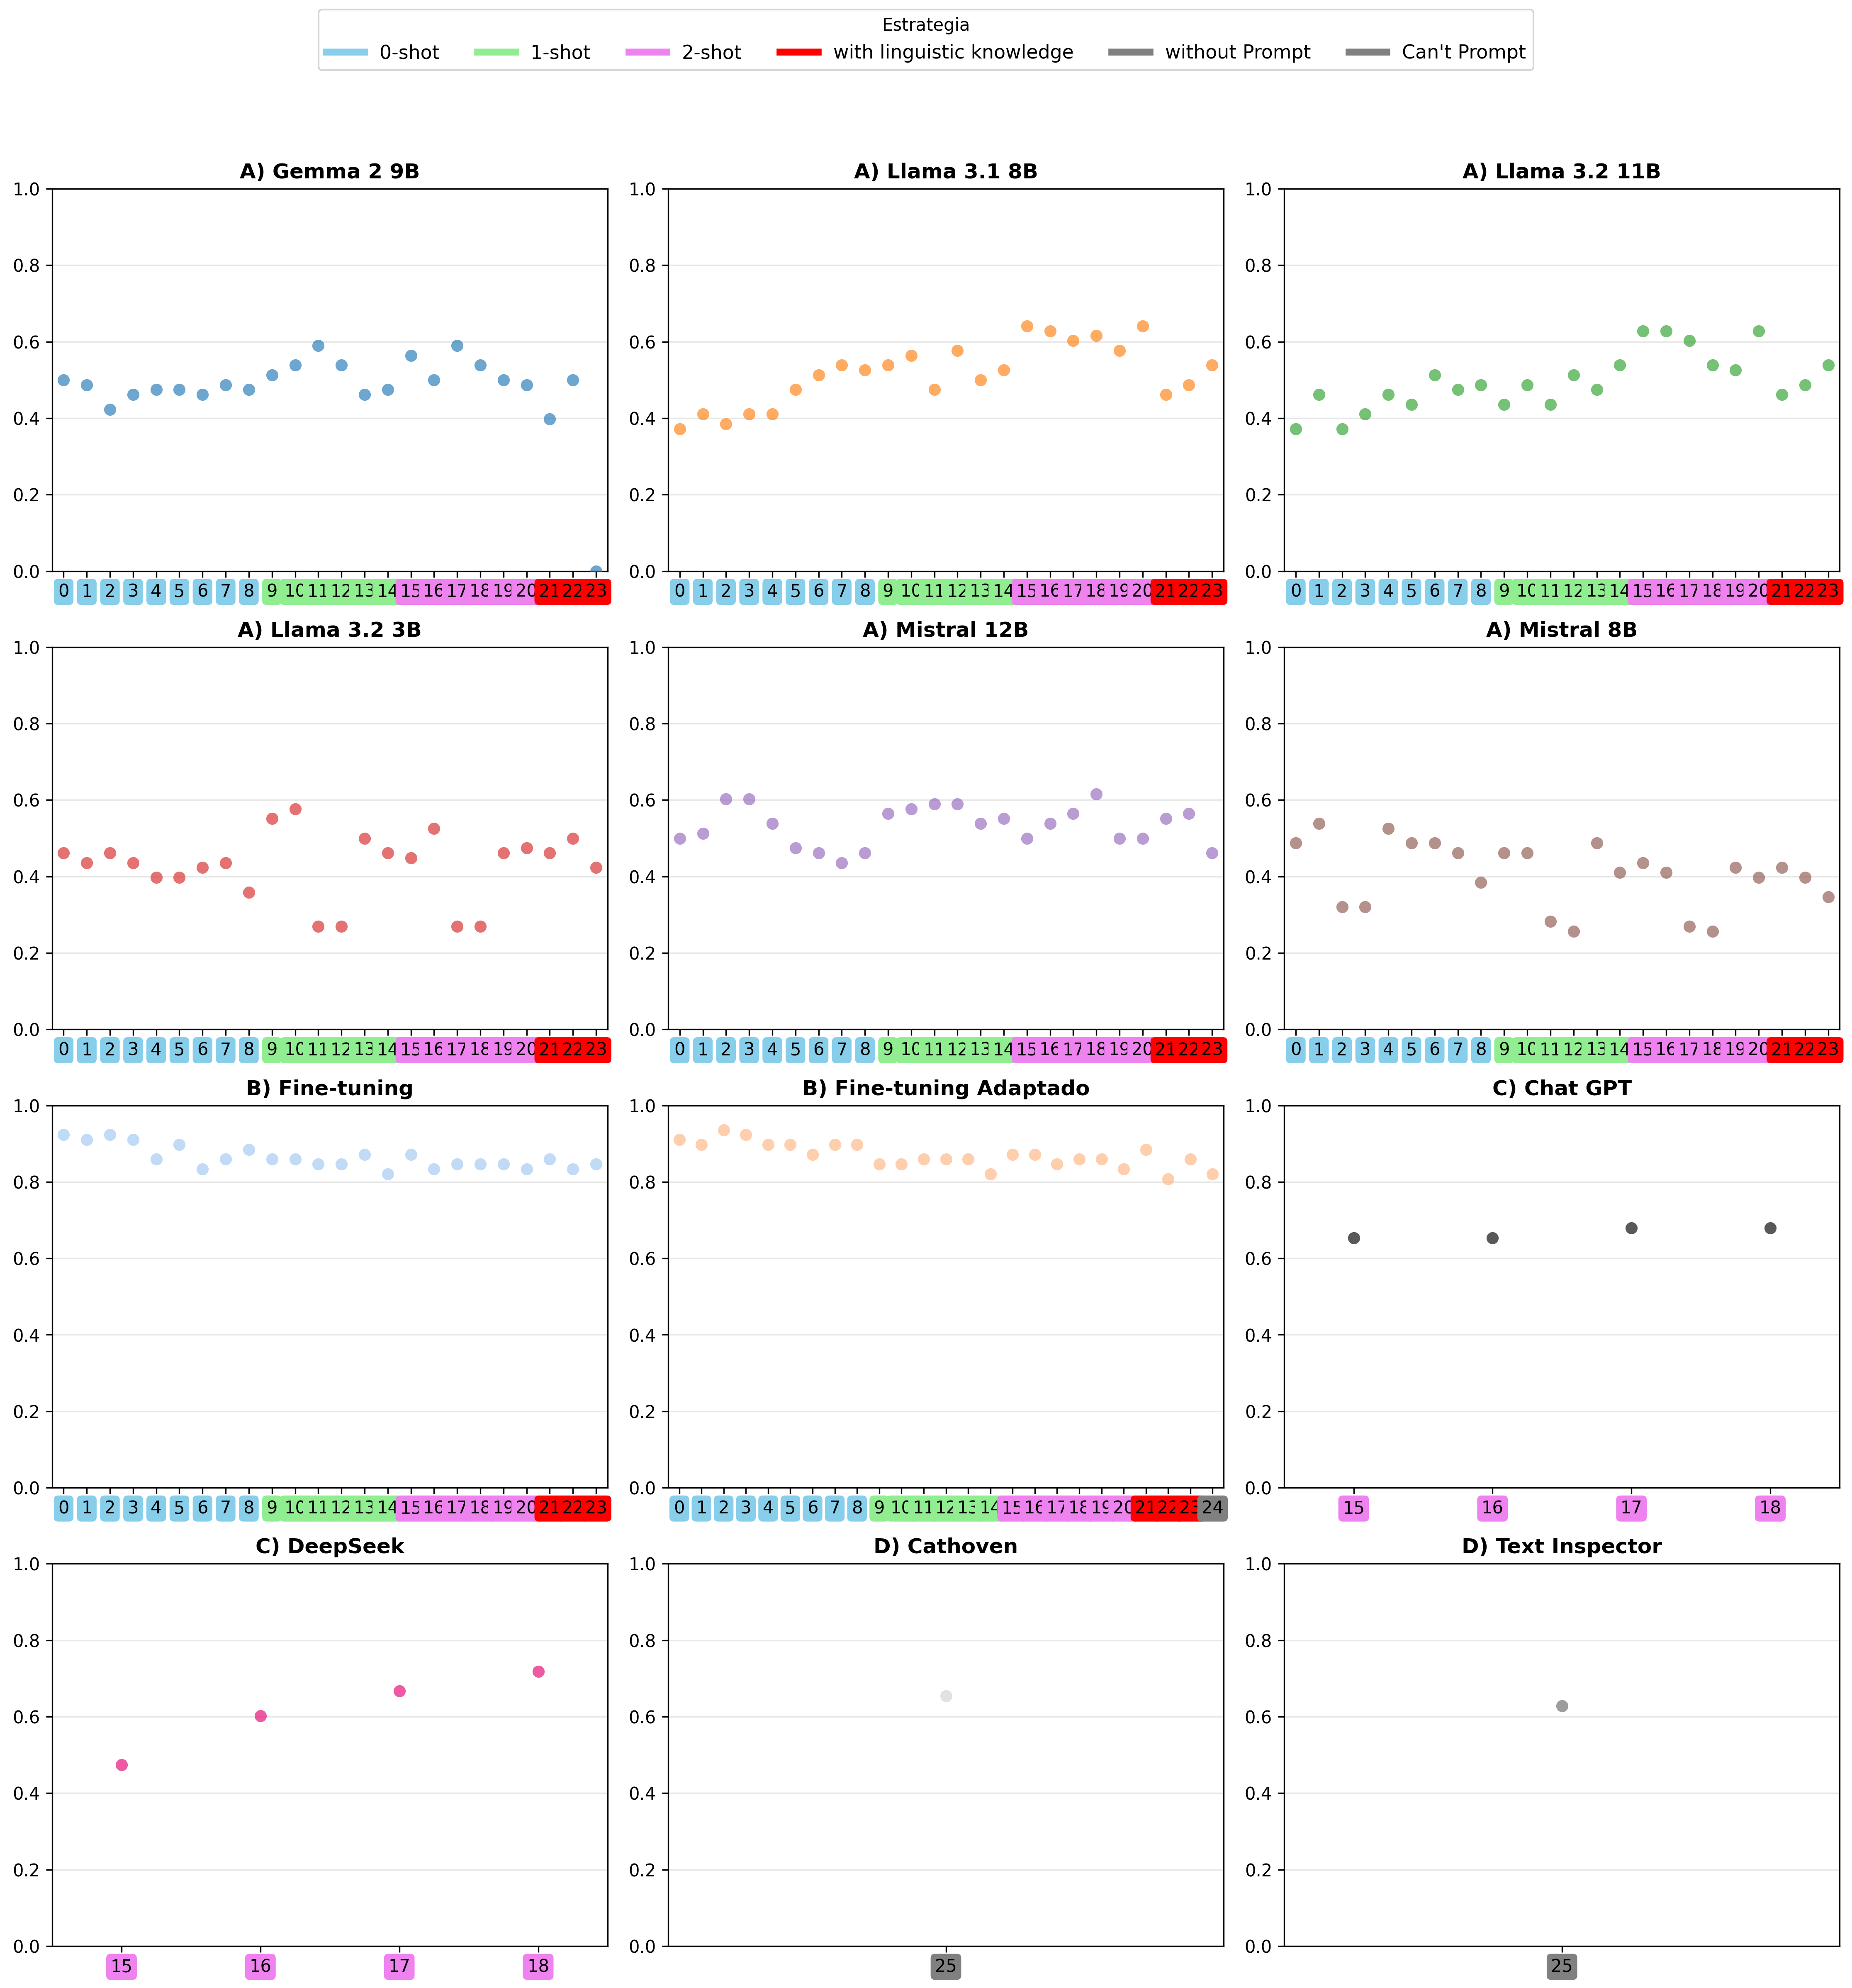
\includegraphics[width=\textwidth]{Graficos Tesis/custom_dataset_evaluacion_stripplot_por_modelo.png}
  \caption{Aproximated Acuraccy de todos los experimentos realizados, separados por modelo.}
  \label{fig:modelos_ind}
\end{figure*}

\todo{cambiar el texto a español}
\todo{cambiar color de cathoven y text inspector}

\noindent\textbf{Análisis de Tablas de resultados}\\
\todo{mejorar esta parte}
Las Tablas \ref{} complementan los análisis visuales con los valores numéricos de accuracy aproximada.
Tabla \ref{} resultados en partición eval (todos los modelos).
Los 10 mejores experimentos están ocupados exclusivamente por variantes del Modelo 1 y Modelo 2 con fine-tuning, con accuracies aproximadas entre 0.91 y 0.94.


El mejor experimento sin fine-tuning aparece en la posición 95 (DeepSeek, experimento 18), siendo la alternativa no ajustada con mejor desempeño.
Esto refuerza la conclusión principal: el fine-tuning genera una mejora sustancial, estable y consistente.

Tabla 3 — Top 10 experimentos sin fine-tuning (partición eval).
Los modelos privativos DeepSeek y ChatGPT dominan los primeros puestos.


Sin embargo, la ventaja respecto de modelos libres no es amplia.


LLaMA 3.1 8B aparece en la posición 8 con una accuracy aproximada de 0.64, muy próxima a la de los modelos privativos.
Este resultado es coherente con la Figura 3, donde los modelos libres presentan mayor variabilidad pero alcanzan niveles competitivos.
Tabla 4 — Top 10 modelos open-source (partición train + eval).
El mejor resultado lo obtiene LLaMA 3.1 8B (experimento 18), con accuracy aproximada de 0.63.


Los tres primeros lugares corresponden a distintas configuraciones del mismo modelo.


El resto de la tabla está compuesto por modelos LLaMA 3.2 11B y Gemma 2 9B, con diferencias menores a 0.04 puntos entre el puesto 1 y el 10.
Esto indica que, con un mayor volumen de textos para la evaluación, los modelos libres presentan un comportamiento más parejo, y que las diferencias de rendimiento están más relacionadas con la estabilidad y la ventana de contexto que con las capacidades intrínsecas de las arquitecturas.\\


\noindent\textbf{Bias de los modelos}\\

Anteriormente mencionamos que existian modelos que tenian un bias hacia categorias particulares, en el grafico \ref{fig:bias} podemos observar que todos los modelos tienen una clase que tiene sobre representacion con respecto de la distribucion original del dataset. Se puede ver que para Llama 3.1 8B, Llama 3.2 11B, Mistral 12B, Chat Gpt y DeepSeek tiene un bias sobre B2, es decir la mayoria de los modelos sin finetuning tiene un bias hacia B2.

Ademas se puede observar las categorias que tienen una baja representacion, como C2 para Gemma 2 9B o A1 para Llama 3.1 8B. Es de esperar que los extremos tengan una baja representacion, pero hay casos distintos como B2 para Llama 3.2 3B y Chat Gpt.

Para el caso de los modelos con finetuning tiene una distribucion mas similar a la original, pero se puede observar que hay una sobre representacion de A2 y baja representacion hacia B1, \textbf{\large esto necesita un estudio particular sobre los textos de la particion de evaluacion que se estan clasificando mal de B1, ya que es posible que sean estructuralemente parecidos a los textos de A2 de la particion de entrenamiento, o sean distintos a los textos de B1 de la particion de entrenamiento. Tambien esta la posibilidad de que se encuentren mal clasificados, ya que no hay una clara distincion entre los niveles.} \\



\begin{figure*}[]
  \centering
  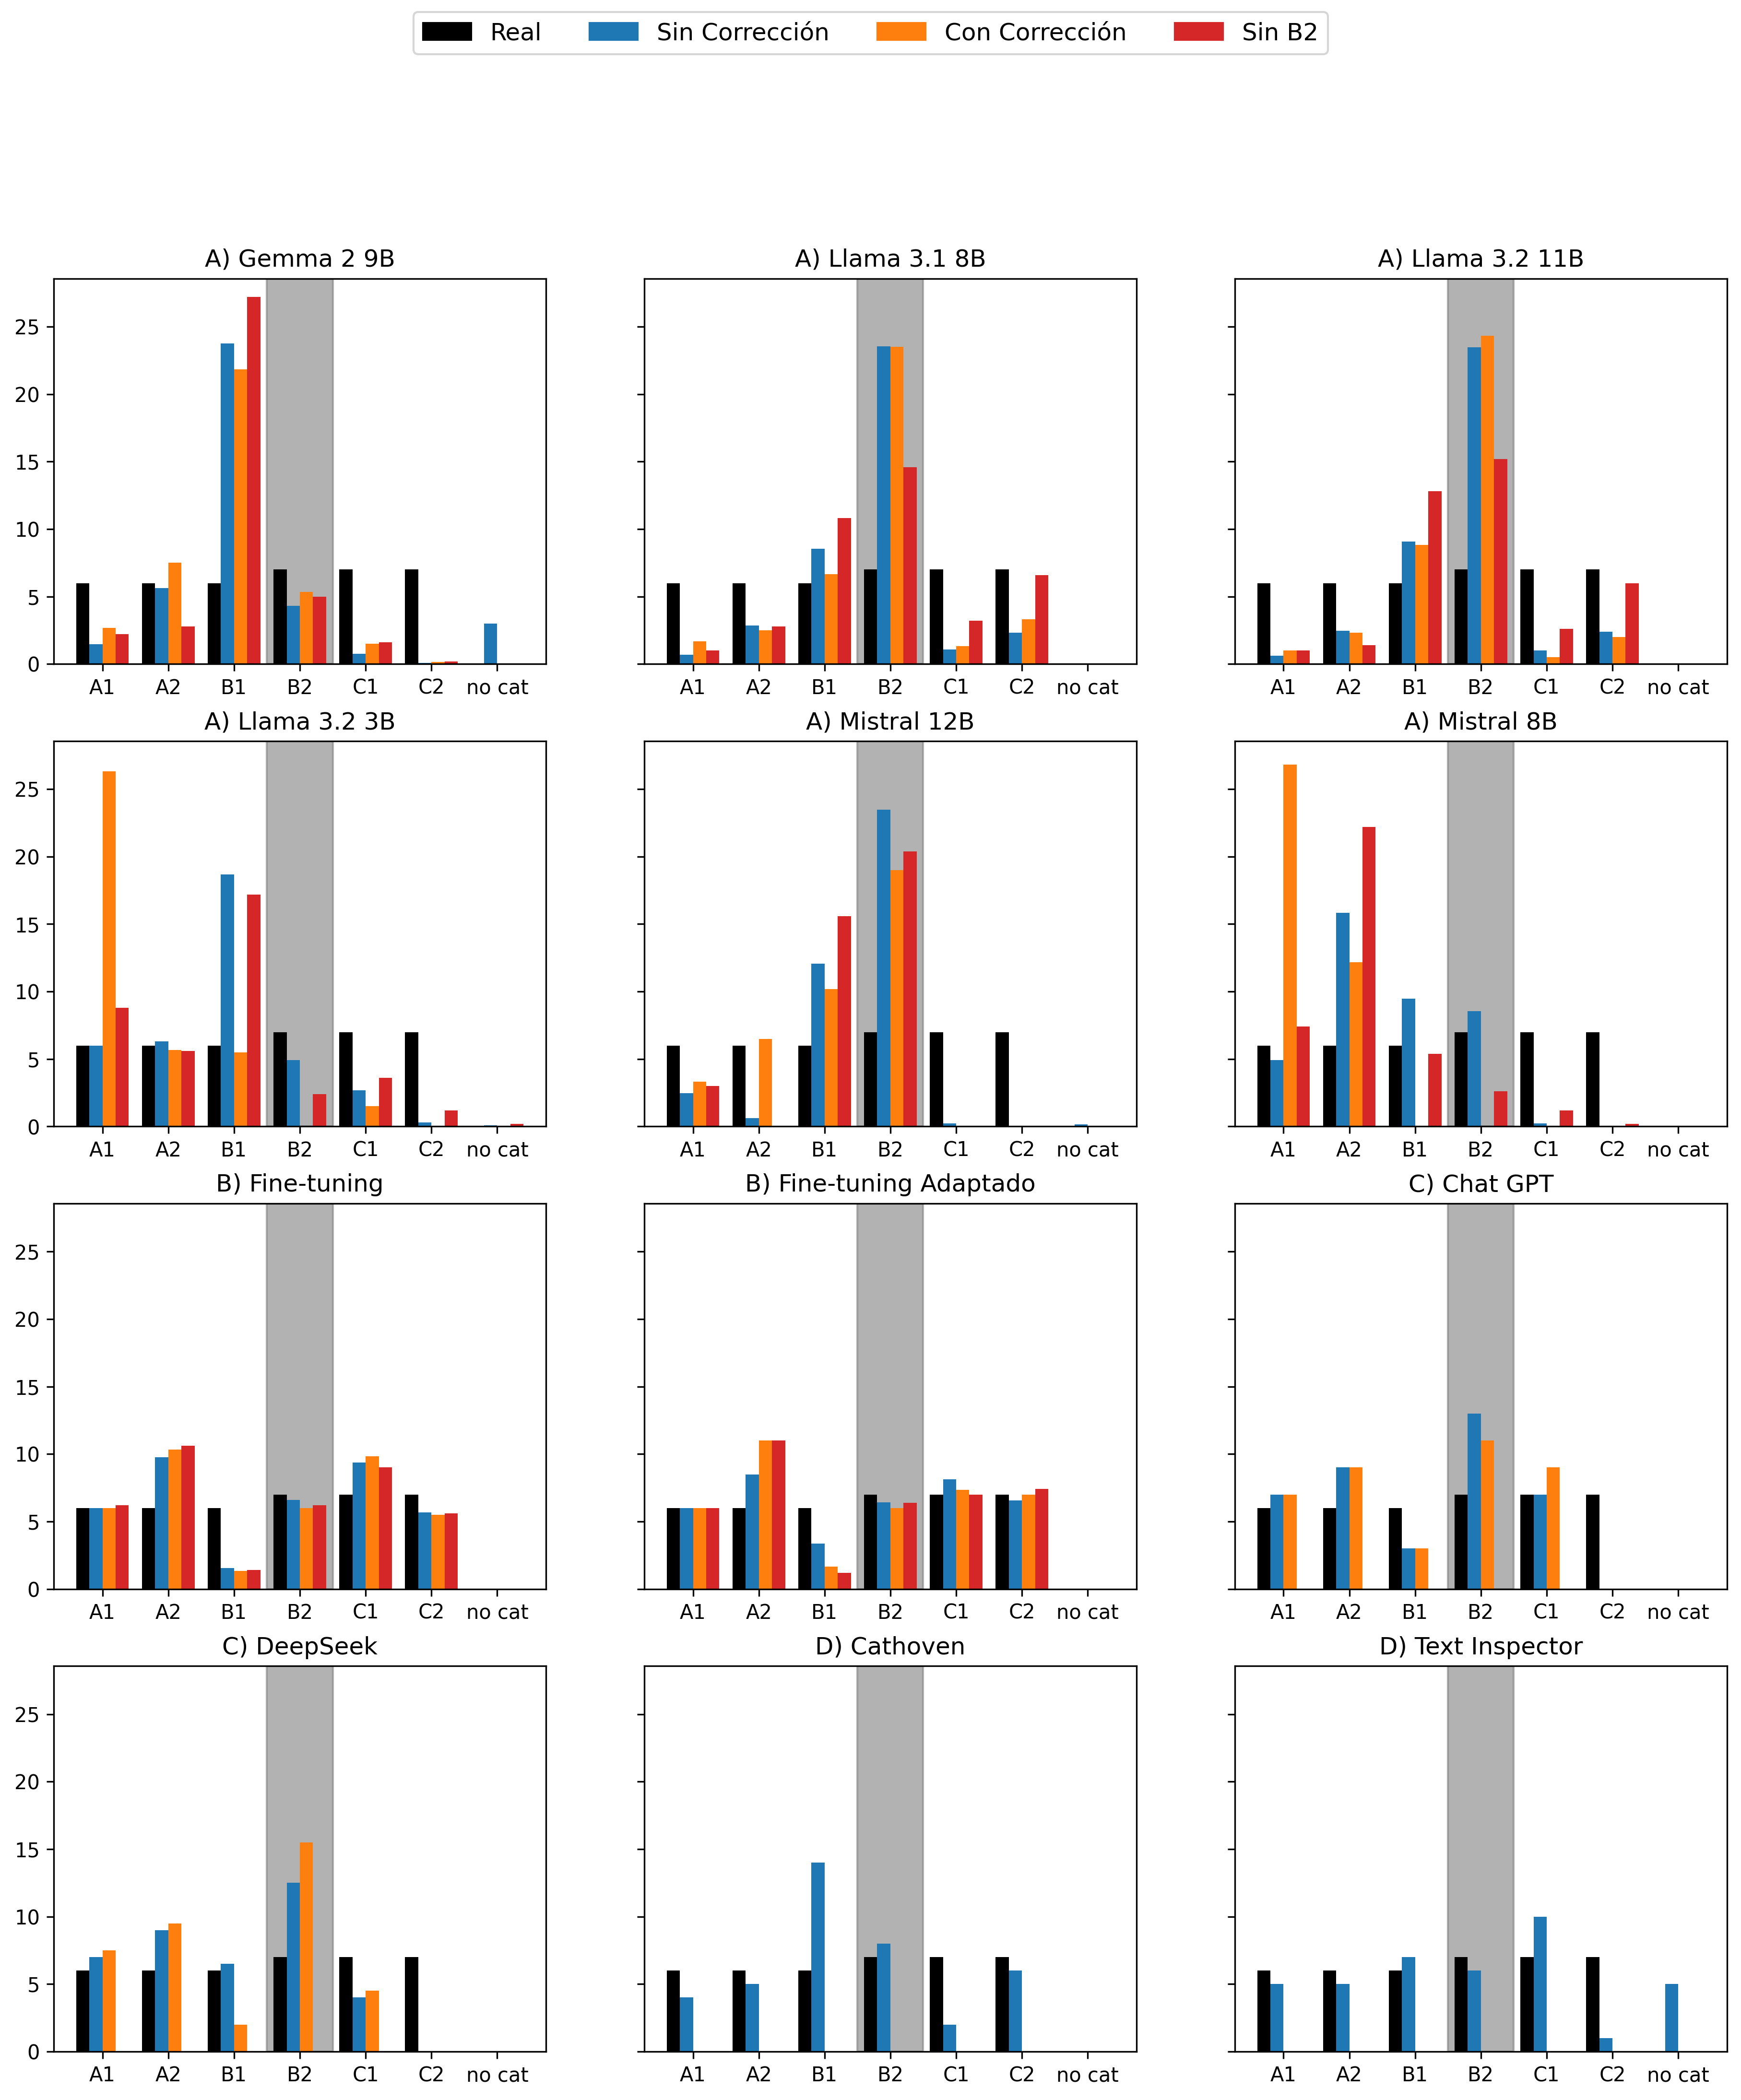
\includegraphics[width=\textwidth]{Graficos Tesis/custom_dataset_evaluacion_bias.png}
  \caption{Cantidad de predicciones promedias hechas por cada modelo, agrupadas por el tipo de prompt. El area de B2 se ecuentra sobreada para una lectura mas facil. No cat significa que no se encontro una clasificacion valida}
  \label{fig:bias}
\end{figure*}
\todo{sacar espacio entre leyenda y imagen, sacar no cat de los que no hacen falta}



